\section{Esercitazione III.}

\begin{enumerate}
\item\begin{itemize}
\item[a)]Dire cosa produce la seguente sequenza di comandi Matlab:
\begin{codice}
\begin{verbatim}
>> x = linspace(-3/2,3/2,300);
>> y = 1-(1-x.^2).^2;
>> plot(x,y);
\end{verbatim}
\end{codice}
\item[b)]Scrivere e stampare un file script di Matlab in grado di generare una 
matrice triangolare superiore $A$ di dimensione $8 \times 8$, con gli elementi
della diagonale principale uguale a $0$, quelli della prima sopradiagonale
uguali a $-1$. quelli della seconda sopradiagonale $-2$ e \ldots quelli
dell'ultima sopradiagonale uguali a $-7$. Quindi ridefinire gli elementi
$A(i,j)$ della parte triangolare inferiore in modo tale che $A(i,j) = -A(j,i)$.
Denotata con $B$ la matrice modificata, verificare se è simmetrica.
\end{itemize}
\begin{svol}
\begin{itemize}
\item[a)]La sequenza di comandi generano un vettore \verb1x1 di elementi
equispaziati da $-\frac{3}{2}$ a $\frac{3}{2}$ ed un vettore \verb1y1 di 
elementi
che rappresentano l'immagine del vettore \verb1x1 attraverso la funzione $f(x)=
1 - (1-x^2)^2$.

Il comando \verb1plot(x,y)1 generano il grafico della funzione.
\begin{figure}[!hc]\begin{center}
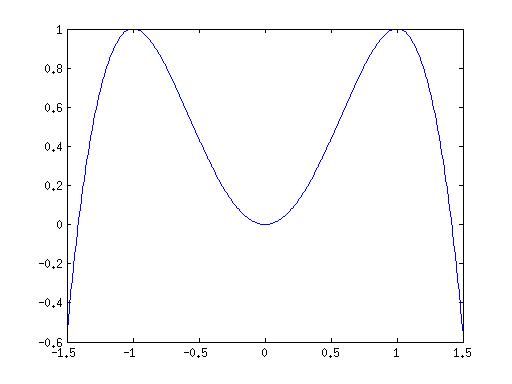
\includegraphics[scale=.35]{fig/es3-1a.jpg}\end{center}
\end{figure}
\item[b)]Il seguente codice è scritto nel file \verb1es3_2.m1 ed è lo script
che opera come richiesto:

\begin{codice}
\begin{verbatim}
A = zeros(8,8);
for i=7:-1:1
  A = A + diag(-i*(ones(i,1)),8-i);
end
\end{verbatim}
\end{codice}
Infatti, stampando la matrice $A$ si ha:
\begin{codice}
\begin{verbatim}
>> A

A =

     0    -7    -6    -5    -4    -3    -2    -1
     0     0    -7    -6    -5    -4    -3    -2
     0     0     0    -7    -6    -5    -4    -3
     0     0     0     0    -7    -6    -5    -4
     0     0     0     0     0    -7    -6    -5
     0     0     0     0     0     0    -7    -6
     0     0     0     0     0     0     0    -7
     0     0     0     0     0     0     0     0

\end{verbatim}
\end{codice}
Si effettua ora la costruzione della matrice $B$ come rischiesto, mediante
una semplice operazione algebrica sulle matrici:
\begin{codice}
\begin{verbatim}
>> B = A - A'

B =

     0    -7    -6    -5    -4    -3    -2    -1
     7     0    -7    -6    -5    -4    -3    -2
     6     7     0    -7    -6    -5    -4    -3
     5     6     7     0    -7    -6    -5    -4
     4     5     6     7     0    -7    -6    -5
     3     4     5     6     7     0    -7    -6
     2     3     4     5     6     7     0    -7
     1     2     3     4     5     6     7     0

>> 
\end{verbatim}
\end{codice}
Ora verifichiamo la simmetria, ricordiamo che una matrice $A$ è simmetrica
se e solo se $A \cdot A^{-1} = I$.
\begin{codice}
\begin{verbatim}
>> B * inv(B)

ans =

    1.0000    0.0000   -0.0000   -0.0000    0.0000   -0.0000    0.0000    0.0000
    0.0000    1.0000   -0.0000   -0.0000    0.0000    0.0000   -0.0000    0.0000
    0.0000         0    1.0000    0.0000   -0.0000    0.0000    0.0000    0.0000
   -0.0000    0.0000   -0.0000    1.0000   -0.0000    0.0000    0.0000   -0.0000
   -0.0000    0.0000   -0.0000   -0.0000    1.0000    0.0000   -0.0000   -0.0000
    0.0000    0.0000    0.0000   -0.0000   -0.0000    1.0000   -0.0000    0.0000
   -0.0000    0.0000   -0.0000   -0.0000         0    0.0000    1.0000   -0.0000
    0.0000   -0.0000    0.0000    0.0000    0.0000         0   -0.0000    1.0000

\end{verbatim}
\end{codice}
La matrice risulta simmetrica.
\end{itemize}
\end{svol}

\item Dopo aver visualizzato in Matlab il valore \verb1realmin1 $\simeq 10^{-m}$,
predisporre e visualizzare in \verb1format long e1 un vettore di $21$ elementi
logaritmicamente equispaziati fra $10^-m$ e $10^{-m-20}$. Commentare i
ruslitati ottenuti.  

\begin{svol}
\begin{codice}
\begin{verbatim}
>> realmin

ans =

  2.2251e-308

>> format long e
>> m = 308;
>> rm = logspace(-m,-m-20,21)

rm =

  Columns 1 through 3

    9.999999999999999e-309    1.000000000000002e-309    9.999999999999969e-311

  Columns 4 through 6

    9.999999999999475e-312    9.999999999984653e-313    1.000000000013287e-313

  Columns 7 through 9

    9.999999999638807e-315    9.999999984816838e-316    9.999999836597144e-317

  Columns 10 through 12

    1.000000230692537e-317    9.999987484955998e-319    9.999888671826830e-320

  Columns 13 through 15

    9.999888671826830e-321    9.980126045993180e-322    9.881312916824931e-323

  Columns 16 through 18

    9.881312916824931e-324                         0                         0

  Columns 19 through 21

                         0                         0                         0

>> 
\end{verbatim}
\end{codice}
Gli elementi del vettore \verb1er1 risultano equispaziati fino al sedicesimo 
elemento, dopodichè si ha il fenomeno di underflow.
\end{svol}

\item
Al variare del parametro $p=10^{\alpha}$, con $\alpha = 1:10$, calcolare mediante
le note formule risolutive, le radici dell'equazione di quarto grado:
\[
x^4 -bx^2 +1 = 0,
\]
con $b = \frac{1+p^2}{p}$. In seguito, dopo aver tradotto tali formule in
istruzioni di assegnazione Matlab, predisporre una tabella con gli errori 
relativi commessi da Matlab nel calcolo numerico delle radici dell'equazione 
assegnata. Motivare i risultati ottenuti.

\begin{svol}Iniziamo a calcolare le radici con le formule note:
\begin{codice}
\begin{verbatim}
>> p = logspace(1,10,10);
>> b = (1+p.^2)./p;
>> 
>> % Per risolvere x^4 -bx^2 + 1 = 0 poniamo t = x^2 e
>> % risolvo l'equazione t^2 - bt + 1 = 0
>> 
>> % Calcolo del delta
>> delta = sqrt(b.^2-4)./2;
>> 
>> % Calcolo dei due possibili valori di t
>> t1 = (b + delta)./2;
>> t2 = (b - delta)./2;
>> 
>> % Calcolo dei valori delle x
>> x1 = sqrt(t1);
>> x2 = -sqrt(t1);
>> x3 = sqrt(t2);
>> x4 = -sqrt(t2);
>>
>> % Inseriamo ora i risultati ottenuti in una tabella X
>> X = [x2' x1' x4' x3']

X =

   1.0e+04 *

  -0.000274317334487   0.000274317334487  -0.000160468065359   0.000160468065359
  -0.000866039837421   0.000866039837421  -0.000500074994376   0.000500074994376
  -0.002738613243961   0.002738613243961  -0.001581141201791   0.001581141201791
  -0.008660254052278   0.008660254052278  -0.005000000075000   0.005000000075000
  -0.027386127875715   0.027386127875715  -0.015811388303214   0.015811388303214
  -0.086602540378458   0.086602540378458  -0.050000000000075   0.050000000000075
  -0.273861278752584   0.273861278752584  -0.158113883008421   0.158113883008421
  -0.866025403784439   0.866025403784439  -0.500000000000000   0.500000000000000
  -2.738612787525831   2.738612787525831  -1.581138830084190   1.581138830084190
  -8.660254037844387   8.660254037844387  -5.000000000000000   5.000000000000000

\end{verbatim}
\end{codice}
Abbiamo così ottenuto una matrice contenente, per ogni riga, le quattro
radici del polinomio al variare del parametro $b$.

Calcoliamo ora le radici con il metodo di Matlab \verb1roots1 e calcoliamo 
l'errore assoluto tra le due soluzioni.
\begin{codice}
\begin{verbatim}
>> for i = 1 : 10
Roots(i,:) = roots([1 0 -b(i) 0 1]);
end
>> Roots

Roots =

   1.0e+05 *

  -0.000031622776602   0.000031622776602  -0.000003162277660   0.000003162277660
  -0.000100000000000   0.000100000000000  -0.000001000000000   0.000001000000000
  -0.000316227766017   0.000316227766017  -0.000000316227766   0.000000316227766
  -0.001000000000000   0.001000000000000  -0.000000100000000   0.000000100000000
  -0.003162277660168   0.003162277660168  -0.000000031622777   0.000000031622777
  -0.010000000000000   0.010000000000000  -0.000000010000000   0.000000010000000
  -0.031622776601684   0.031622776601684  -0.000000003162278   0.000000003162278
  -0.100000000000000   0.100000000000000  -0.000000001000000   0.000000001000000
  -0.316227766016838   0.316227766016838  -0.000000000316228   0.000000000316228
  -1.000000000000000   1.000000000000000   0.000000000100000  -0.000000000100000

>> Ea = abs(X-Roots)

Ea =

   1.0e+04 *

   0.000041910431530   0.000041910431530   0.000128845288757   0.000128845288757
   0.000133960162579   0.000133960162579   0.000490074994376   0.000490074994376
   0.000423664416207   0.000423664416207   0.001577978924130   0.001577978924130
   0.001339745947722   0.001339745947722   0.004999000075000   0.004999000075000
   0.004236648725969   0.004236648725969   0.015811072075448   0.015811072075448
   0.013397459621542   0.013397459621542   0.049999900000075   0.049999900000075
   0.042366487264254   0.042366487264254   0.158113851385645   0.158113851385645
   0.133974596215562   0.133974596215562   0.499999990000000   0.499999990000000
   0.423664872642549   0.423664872642550   1.581138826921912   1.581138826921912
   1.339745962155612   1.339745962155615   5.000000001000000   5.000000001000000

>> 
\end{verbatim}
\end{codice}
Errore relativo:
\begin{codice}
\begin{verbatim}
>> Er = abs((Roots-X)./X)

Er =

   0.152780835408468   0.152780835408469   0.802934144367142   0.802934144367141
   0.154681293851390   0.154681293851391   0.980002999325169   0.980002999325169
   0.154700345929209   0.154700345929209   0.998000002999993   0.998000002999993
   0.154700536454750   0.154700536454750   0.999800000003000   0.999800000003000
   0.154700538360007   0.154700538360007   0.999980000000003   0.999980000000003
   0.154700538379059   0.154700538379060   0.999998000000000   0.999998000000000
   0.154700538379250   0.154700538379250   0.999999800000000   0.999999800000000
   0.154700538379252   0.154700538379252   0.999999980000000   0.999999980000000
   0.154700538379252   0.154700538379252   0.999999998000000   0.999999998000000
   0.154700538379251   0.154700538379252   1.000000000200000   1.000000000200000

>> 
\end{verbatim}
\end{codice}
\end{svol}

\item In relazione al calcolo numerico della derivata di $f(x) = e^x$, in
$x = 1$, si considerino le seguenti approssimazioni:
\[
\frac{f(x+h)-f(x)}{h}, \ \frac{f(x+h)-f(x-h)}{2h}.
\]
Si indichi l'errore analitico per entrambe le discretizzazioni cosiderate
e si predispongano con Matlab, al variare del parametro $h = 10^{-\alpha}$,
$\alpha = 1, \ldots, 20$:
\begin{itemize}
\item[a)]una tabella in \verb1format short e1 contenente i valori di $h$ e i
corrispondenti errori analitici;
\item[b)]un grafico di tali errori in scala logaritmica.
\end{itemize}
Analizzare i risultati ottenuti.

\begin{svol}
\begin{itemize}
\item[a)]
Poniamo \verb1e1 come il valore $e^x$, con $x = 1$ e calcoliamo i valori delle
approssimazioni \verb1p1 utilizzando i parametri indicati.
\begin{codice}
\begin{verbatim}
>> e = exp(1);
>> for i=1:20
h(i) = 10^(-i);
end
>> 
>> p1 = (exp(1+h)-e)./h;
>> p2 = (exp(1+h)-exp(1-h))./(2*h);
>> 
>> e1 = e -p1;
>> e2 = e -p2;
>> 
>> O = [h; e1; e2];
>> fprintf('%e \t %e \t %e \n',O)
1.000000e-01 	 -1.405601e-01 	 -4.532735e-03 
1.000000e-02 	 -1.363683e-02 	 -4.530492e-05 
1.000000e-03 	 -1.359594e-03 	 -4.530467e-07 
1.000000e-04 	 -1.359186e-04 	 -4.530565e-09 
1.000000e-05 	 -1.359145e-05 	 -5.858736e-11 
1.000000e-06 	 -1.358527e-06 	 1.634577e-10 
1.000000e-07 	 -1.355058e-07 	 -5.858691e-11 
1.000000e-08 	 5.101167e-08 	 6.602751e-09 
1.000000e-09 	 2.286474e-07 	 6.602751e-09 
1.000000e-10 	 2.893183e-06 	 6.727366e-07 
1.000000e-11 	 1.177497e-05 	 -1.042949e-05 
1.000000e-12 	 1.177497e-05 	 -2.102696e-04 
1.000000e-13 	 4.896756e-03 	 4.558642e-04 
1.000000e-14 	 5.374657e-02 	 9.337648e-03 
1.000000e-15 	 5.374657e-02 	 -1.682980e-01 
1.000000e-16 	 2.718282e+00 	 4.978358e-01 
1.000000e-17 	 2.718282e+00 	 2.718282e+00 
1.000000e-18 	 2.718282e+00 	 2.718282e+00 
1.000000e-19 	 2.718282e+00 	 2.718282e+00 
1.000000e-20 	 2.718282e+00 	 2.718282e+00 
>> 
\end{verbatim}
\end{codice}

\end{itemize}
\end{svol}

\item
Usando il comando Matlab \verb1Hilb(n)1 costruire la matrice di Hilbert di 
ordine $10$. Costruire poi il vettore $b$ in modo che il sistema lineare 
$Hx = b$ abbia solunzione il vettore $x$ con tutte le componenti uguali a $1$.

Risolvere il sistema lineare $Hx = b$ usando i comandi Matlab. Costruire poi il
vettore $c= b + z$ dove $z^t = [0.001 0 \cdots 0]$ e risolvere il nuovo sistema
$Hy = c$.

Calcolare $e_r = \frac{\|x-y\|_2}{\|x\|_2} $.

\begin{svol}
Calcloiamo $H$ utilizzando il comando specificato, e mediante operazioni
elementari ricaviamo il vettore $b$ e quindi $x$.
\begin{codice}
\begin{verbatim}
>> H = hilb(10);
>> b = H*ones(10,1);
>> 
>> x = H\b

x =

   0.999999998715226
   1.000000110249369
   0.999997664058654
   1.000021147216568
   0.999899477767458
   1.000275541218743
   0.999549027556600
   1.000434891240842
   0.999772107416504
   1.000050035409456

>> 
\end{verbatim}
\end{codice}
Come si può notare il vettore $x$ è perturbato da errori algoritmici.

\begin{codice}
\begin{verbatim}
>> z = [0.001; zeros(9,1)];
>> c = b+z

c =

   2.929968253968254
   2.019877344877345
   1.603210678210678
   1.346800421800422
   1.168228993228993
   1.034895659895660
   0.930728993228993
   0.846695379783615
   0.777250935339171
   0.718771403175428

>> y = H\c

y =

   1.0e+03 *

   0.001099997010956
  -0.003949743297673
   0.080194557919823
  -0.599550712574902
   2.523285644515019
  -6.304657469284754
   9.609548217661349
  -8.749585606735506
   4.376268391416600
  -0.922663274650903

>> er = norm(x-y)/norm(x)

er =

     4.851631507736105e+0
\end{verbatim}
\end{codice}
\end{svol}

\end{enumerate}

\section{Esercitazione IV.}

\begin{enumerate}
\item
\begin{itemize}
\item[a)]Rappresentare graficamente su un intervallo $[a,b]$ la funzione
\[f(x) = 2 \sin(8x)-\ln(x^2+1)\]
usando una griglia di punti equispaziati dell'intervallo $[a,b]$.
\item[b)]Rappresentare la funzione $f(x)$ definita da:
\[f(x) = \left\{\begin{array}{lr}x^2&x\leq 3\\9&x > 3\end{array}\right.\]
sull'intervallo $[2,4]$.
\end{itemize}

\begin{svol}
\begin{itemize}
\item[a)]Svolgiamo l'esercizio utilizzando due griglie di punti ed usiamo
il comando \verb1plot1 per visualizzare i due grafici in una sola figura.
Cogliamo l'occasione per vedere la differenza di rappresentazione
di una funzione in base alla scelta del numero di punti.
\begin{codice}
\begin{verbatim}
>> % Definiamo il nostro intervallo [a,b] come per
>> % per il punto b), ovvero a = 2 e b = 4.
>> a = 2;
>> b = 4;
>> x = linspace(a,b,1000); 
>> 
>> % Calcoliamo ora la f(x) del punto a)
>> Fxa = 2*sin(8*x)-log(x.^2 +1);
>> 
>> % Proviamo ora a utilizzare una griglia con meno punti, per poi
>> % confrontarne i grafici.
>> x1 = linspace(a,b,20);
>> ya = 2*sin(8*x1)-log(x1.^2 +1);
>> 
>> % Stampa dei due grafici.
>> plot(x,Fxa,x1,ya,'r')
\end{verbatim}
\end{codice}
\begin{figure}[!ht]\begin{center}
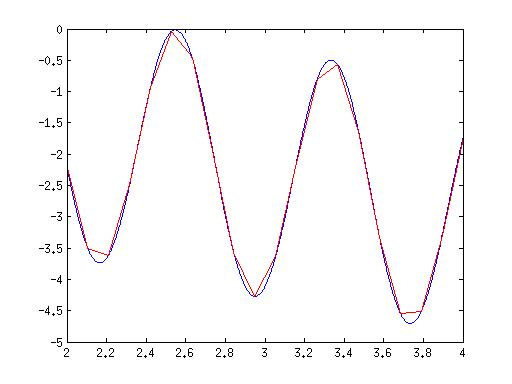
\includegraphics[scale=.50]{fig/es4-1a.jpg}\end{center}
\caption{esercizio $1$.a}
\end{figure}

\item[b)]Analogamente al punto a) vediamo due griglie.
\begin{codice}
\begin{verbatim}
>> % Calcoliamo ora l'intervallo per la funzione f(x) per il punto
>> % b) suddividendola in due intervalli x = x1b U x2b
>> x1b = linspace(2,3,500);
>> x2b = linspace(3,4,500);
>> 
>> % Calcoliamo ora i valori della funzione definita a tratti, escludendo il
>> % primo punto del primo vettore.
>> fxb1 = x1b.^2;
>> fxb2 = 9*ones(1,500);
>> 
>> % Ripetiamo i calcoli utilizzando meno punti.
>> x1bb = linspace(2,3,10);
>> x2bb = linspace(3,4,10);
>> 
>> fxbb1 = x1bb.^2;
>> fxbb2 = 9*ones(1,10);
>> 
>> % Stampiamo i grafici facendo attenzione ad escludere il primo punto
>> % della seconda parte del vettore.
>> plot(x1b,fxb1,x2b(2:500),fx2b(2:500), x1bb,fx1bb,'r',x2bb(2:10),fxbb2(2:10),'r')
??? Undefined function or method 'fx2b' for input arguments of type 'double'.
 
>> plot(x1b,fxb1,x2b(2:500),fxb2(2:500), x1bb,fx1bb,'r',x2bb(2:10),fxbb2(2:10),'r')
??? Undefined function or variable 'fx1bb'.
 
>> plot(x1b,fxb1,x2b(2:500),fxb2(2:500), x1bb,fxbb1,'r',x2bb(2:10),fxbb2(2:10),'r')
>> 
\end{verbatim}
\end{codice}
\begin{figure}[!ht]\begin{center}
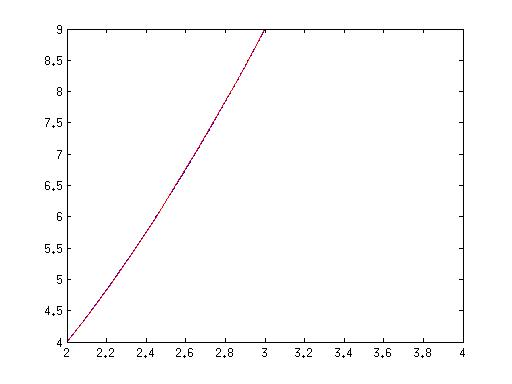
\includegraphics[scale=.50]{fig/es4-1b.jpg}\end{center}
\caption{esercizio $1$.b}
\end{figure}

\end{itemize}
\end{svol}

\item 
\begin{itemize}
\item[a)]
Dopo aver visualizzato in Matlab il valore \verb1realmin1 $\simeq 10^{-m}$,
predisporre e visualizzare in formato \verb1format long e1 un vettore di
$21$ elementi logaritmicamente equispaziati fra $10^{-m}$ e $10^{-m-20}$.
\item[b)]Visualizzare i valori \verb1realmax1, \verb1realmax1$\cdot 10$,
\verb1realmax1$\cdot (1+eps)$.
\item[c)]Visualizzare i valori $1+10^{-17}$ e $1 + 10^{17}$.
\end{itemize}

\begin{svol}
\begin{enumerate}
\item[a)]
\begin{codice}
\begin{verbatim}
>> format long e
>> realmin

ans =

    2.225073858507201e-308

>> logspace(-m,-m-20,21)'

ans =

    9.999999999999999e-309
    1.000000000000002e-309
    9.999999999999969e-311
    9.999999999999475e-312
    9.999999999984653e-313
    1.000000000013287e-313
    9.999999999638807e-315
    9.999999984816838e-316
    9.999999836597144e-317
    1.000000230692537e-317
    9.999987484955998e-319
    9.999888671826830e-320
    9.999888671826830e-321
    9.980126045993180e-322
    9.881312916824931e-323
    9.881312916824931e-324
                         0
                         0
                         0
                         0
                         0

\end{verbatim}
\end{codice}{\samepage
Con il comando \verb1logspace1 troviamo alcuni valori più piccoli di
\verb1realim1, che ricordiamo, è il più piccolo numero \emph{normalizzato} in
doppia precisione rappresentabile. Come si può vedere infatti, i numeri
trovati non sono normalizzati (non iniziano con un $1$ prima della virgola 
oppure hanno più zeri subito dopo) e di conseguenza è possibile utilizzare
più \verb1bits1 per l'esponente (o caratteristica) e meno per la mantissa.
Ad un certo punto la caratteristica esce comunque dal range ($p<-m$) e si
ha quindi il fenomeno dell'underflow.}
\item[b)]Valutiamo i seguenti risultati:
\begin{codice}
\begin{verbatim}
>> realmax

ans =

    1.797693134862316e+308

>> realmax*10

ans =

   Inf

>> realmax*(1+eps)

ans =

   Inf
\end{verbatim}
\end{codice}
Abbiamo qui il fenomeno di overflow.

\item[c)]
\begin{codice}
\begin{verbatim}
>> 1+10^17

ans =

     1.000000000000000e+17

>> 1+10^-17

ans =

     1

>> 
\end{verbatim}
\end{codice}
In questi due casi abbiamo il fenomeno di arrotondamento, e poiché
gli addendi di $1$ sono minori di $\frac{\beta}{2}$ i risultati
vengono troncati.
\end{enumerate}
\end{svol}

\item
Scrivere un file script in Matlab in grado di calcolare la ``precisione di
macchina'' in base $2$, ricordando che tale valore è caratterizzato come il 
più piccolo numero macchina positivo tale che $fl(1+eps) >1$.

\begin{svol}Lo script Matlab, salvato in un file di nome \verb1epsilon.m1
è il seguente:
\begin{codice}
\begin{verbatim}
epsi =1;
while (1+epsi)>1
    epsi = (1/2)*epsi;
end
epsi=epsi*2
\end{verbatim}
\end{codice}
Richiamando lo script nell'ambiente di lavoro si ha il seguente risultato:
\begin{codice}
\begin{verbatim}
>> eps

ans =

   2.2204e-16

>> epsilon

epsi =

   2.2204e-16

>> 
\end{verbatim}
\end{codice}
\end{svol}

\item
Vedere esercizio $3$ della terza esercitazione.

\item
Osservare l'andamento del resto nello sviluppo di Taylor seguente:
\[
\sin(x+1) = \sin(1) + \cos(1)\cdot x + R(x).
\]
Fare un grafico in scala logaritmica dell'andamento del resto in funzione
di $x$.

\begin{svol}
Per vedere l'andamento del resto, otteniamo mediante operazioni algebriche
i valori di $R(x) = s\in(x+1) - (\sin(1) +\cos(1)\cdot x$ su un'intervallo di 
punti logaritmicamente equispaziati.
\begin{codice}
\begin{verbatim}
>> x = logspace(-13,0,1000);
>> 
>> % Calcolo di R(x)
>> R = sin(x+1) - (sin(1) + cos(1).*x);
>> 
>> plot(x,R)
>> 
\end{verbatim}
\end{codice}


\begin{figure}[!ht]\begin{center}
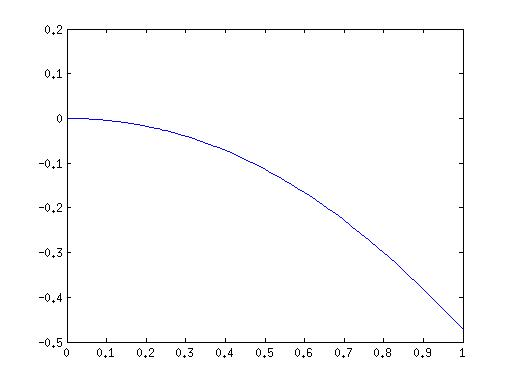
\includegraphics[scale=.50]{fig/es4-5.jpg}\end{center}
\caption{esercizio $5$}
\end{figure}
\end{svol}

\item Osservare la convergenza nel calcolo dei limiti delle seguenti
funzioni:
\begin{itemize}
\item $x \cdot (\sqrt{(x^2+1)}-x)$;
\item $x \cdot \sqrt{(x^2+1)}-x^2$;
\item $x / (\sqrt{(x^2+1)}+x)$.
\end{itemize}

\begin{svol}
Come nell'esercizio della sezione \ref{esercizio4-6} dedicata ai test
campione, si può notare che il limite a $+\infty$ tende ad $\frac{1}{2}$.
\begin{codice}
\begin{verbatim}
>> x = logspace(-13,0,15);
>> 
>> f1 = x.*(sqrt(x.^2 + 1)-x);
>> f2 = x.*sqrt(x.^2+1)-x.^2;
>> f3 = x./(sqrt(x.^2 + 1) +x);
>> 
>> % Creo un vettore di output y (matrice)
>> y = [x; f1; f2; f3];
>> 
>> % funzione di stampa
>> format long e
>> fprintf('%.3e %18.16f %18.16f %18.16f \n',y)
1.000e-13 0.0000000000001000 0.0000000000001000 0.0000000000001000 
8.483e-13 0.0000000000008483 0.0000000000008483 0.0000000000008483 
7.197e-12 0.0000000000071969 0.0000000000071969 0.0000000000071969 
6.105e-11 0.0000000000610540 0.0000000000610540 0.0000000000610540 
5.179e-10 0.0000000005179475 0.0000000005179475 0.0000000005179475 
4.394e-09 0.0000000043939705 0.0000000043939705 0.0000000043939705 
3.728e-08 0.0000000372759358 0.0000000372759358 0.0000000372759358 
3.162e-07 0.0000003162276660 0.0000003162276660 0.0000003162276660 
2.683e-06 0.0000026826885984 0.0000026826885984 0.0000026826885984 
2.276e-05 0.0000227579413192 0.0000227579413192 0.0000227579413192 
1.931e-04 0.0001930325005496 0.0001930325005496 0.0001930325005496 
1.638e-03 0.0016352132081426 0.0016352132081426 0.0016352132081426 
1.389e-02 0.0137032264540035 0.0137032264540035 0.0137032264540035 
1.179e-01 0.1047980301759449 0.1047980301759449 0.1047980301759449 
1.000e+00 0.4142135623730951 0.4142135623730951 0.4142135623730951 
\end{verbatim}
\end{codice}
Intuitivamente dai valori della tabella stampata sulla command window il limite
tende a $0$, vediamo un grafico tabulando con $1000$ punti ancora più
vicini a a $0$.
\begin{codice}
\begin{verbatim}
>> x = logspace(-15,0,1000);
>> f1 = x.*(sqrt(x.^2 + 1)-x);
>> f2 = x.*sqrt(x.^2+1)-x.^2;
>> f3 = x./(sqrt(x.^2 + 1) +x);
>> plot(x,f1)
>> xlabel('x')
>> 
>> plot(x,f1)
>> xlabel('asse delle ascisse')
>> 
\end{verbatim}
\end{codice}

\begin{figure}[!ht]\begin{center}
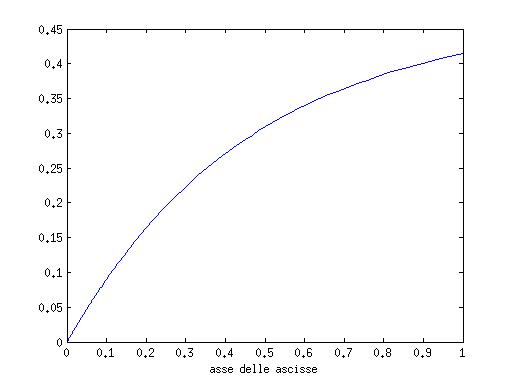
\includegraphics[scale=.50]{fig/es4-6.jpg}\end{center}
\caption{esercizio $6$, si può notare che $\displaystyle \lim_{x \to o}f(x)=0$.}
\end{figure}

\end{svol}
\end{enumerate}
